\section{Постановка задачи}

\begin{frame}[t]{Исследование пещер}


    \begin{columns}[T,onlytextwidth]
        \begin{column}{0.62\textwidth}
            \small
                \textbf{Назначение} --- геологоразведка, изучение подземных экосистем
            \begin{exampleblock}{Непроходимые места для человека}
                \begin{itemize}
                    \item Узкие галереи, огромные пропасти, обвалы, сифоны
                    \item Скопление угарного газа
                    \item Потеря ориентации в пространстве
                \end{itemize}
            \end{exampleblock}
            \vspace{-0.2cm}
            \begin{alertblock}{Организации, исследующие пещеры}
                \begin{enumerate}
                    \item \textit{Ученые} --- Горный институт Уральского отделения РАН, Университет Минас-Жерайса, Фонд Бруно Кесслера
                    \item \textit{Космические агентства} --- ESTEC (DAEDALUS), Роскосмос (FEDOR), NASA (CADRE)
                    \item \textit{Военные} --- Darpa Subterranean Challenge
                \end{enumerate}
            \end{alertblock}
        \end{column}
        \begin{column}{0.37\textwidth}
            \vspace{0.025cm}
            \begin{figure}[H]
                \begin{subfigure}{0.49\textwidth}
                    \centering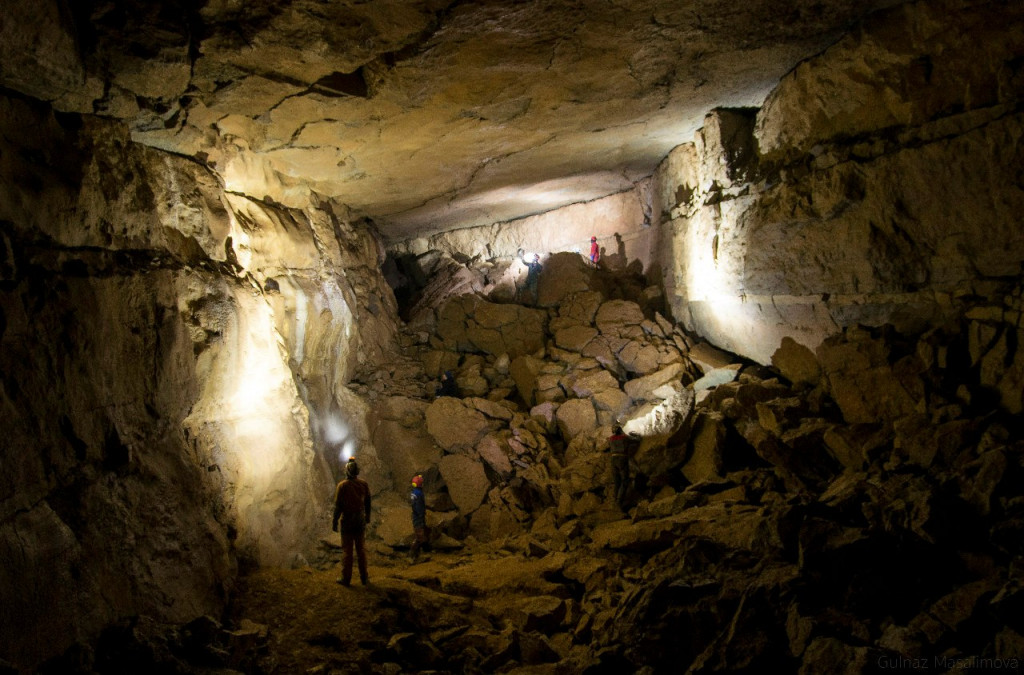
\includegraphics[height=1.75cm,width=1\textwidth,keepaspectratio]{../images/slides/rip.jpg}
                    \caption*{Завал}
                \end{subfigure}
                \begin{subfigure}{0.49\textwidth}
                    \centering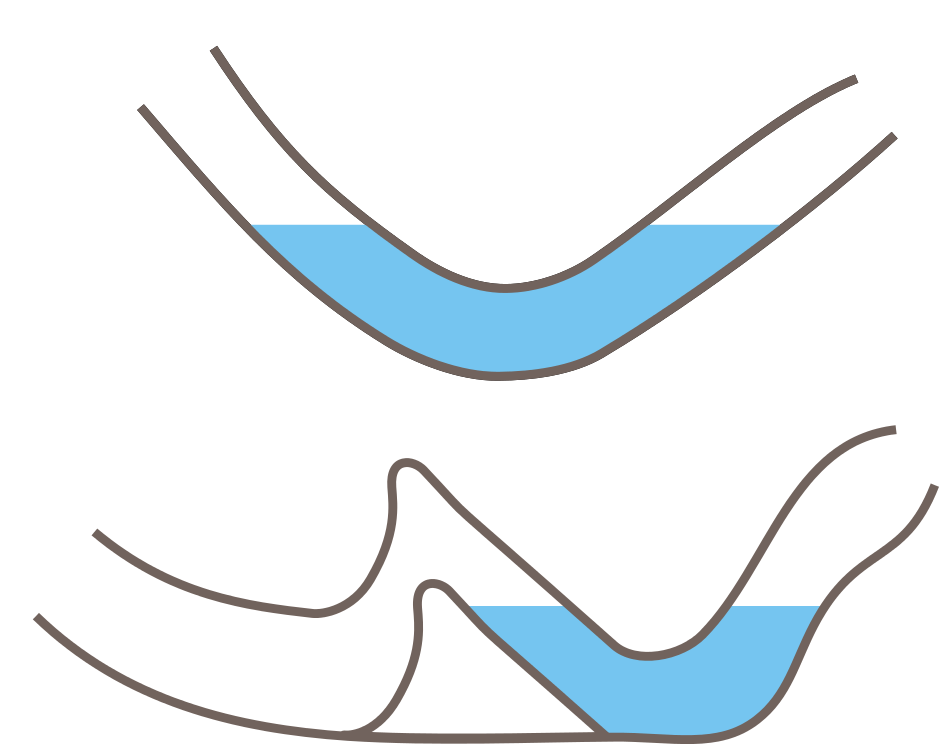
\includegraphics[height=1.75cm,width=1\textwidth,keepaspectratio]{../images/surface_types/siphon.png}
                    \caption*{Сифоны}
                \end{subfigure}
            
                \begin{subfigure}{0.49\textwidth}
                    \centering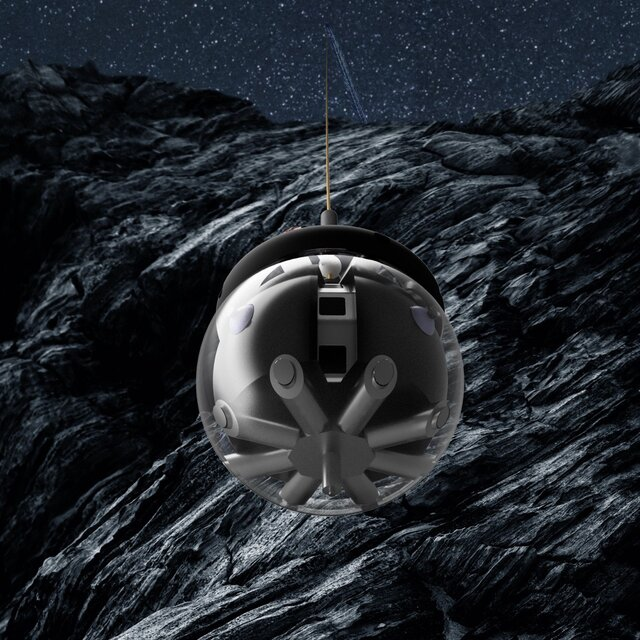
\includegraphics[height=2cm,width=1\textwidth,keepaspectratio]{../images/slides/daedalus.jpg}
                    \caption*{DAEDALUS для исследования пещер на луне}
                \end{subfigure}
                \begin{subfigure}{0.49\textwidth}
                    \centering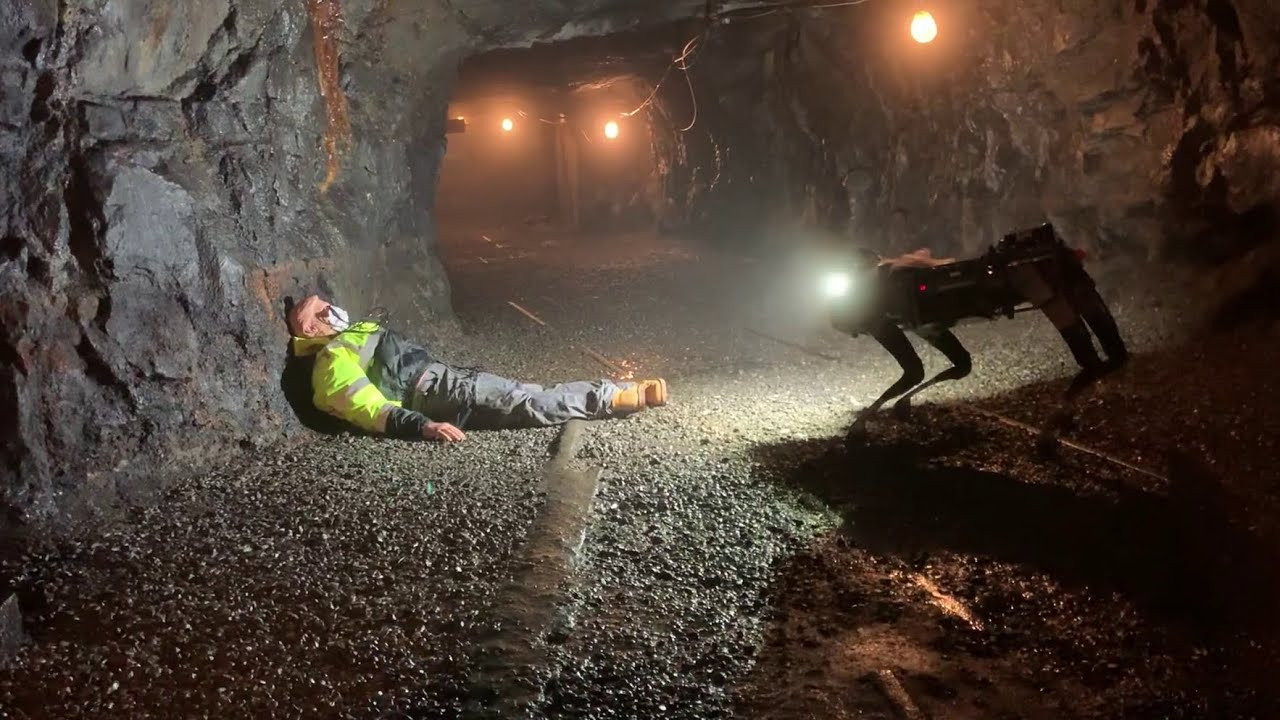
\includegraphics[height=2cm,width=1\textwidth,keepaspectratio]{../images/open_cave.jpg}
                    \caption*{DARPA Subterranean Challenge}
                \end{subfigure}
            \end{figure}
        \end{column}
    \end{columns}
\end{frame}

\note{
\small \setlength{\parindent}{20pt}
\begin{itemize}
    \item Одним из способов нахождения новых минералов или форм жизни является исследование пещер спелеологами. Но данное мероприятие очень опасно, так как
    \item Поэтому разные организации во всем мире пытаются начать применять роботов при исследовании пещер
\end{itemize}  
 }

\begin{frame}[t]{Характеристики пещер}
    \framesubtitle{}
    \vspace{-0.8cm}
    \begin{figure}[H]
        \begin{subfigure}{0.49\textwidth}
            \begin{subfigure}[b]{0.49\textwidth}
                \centering\includegraphics[height=2.2cm,width=1\textwidth,keepaspectratio,page=1]{./tikz_pictures.pdf}
                \caption{Малый водоем}
            \end{subfigure}
            \hfill
            \begin{subfigure}[b]{0.49\textwidth}
                \centering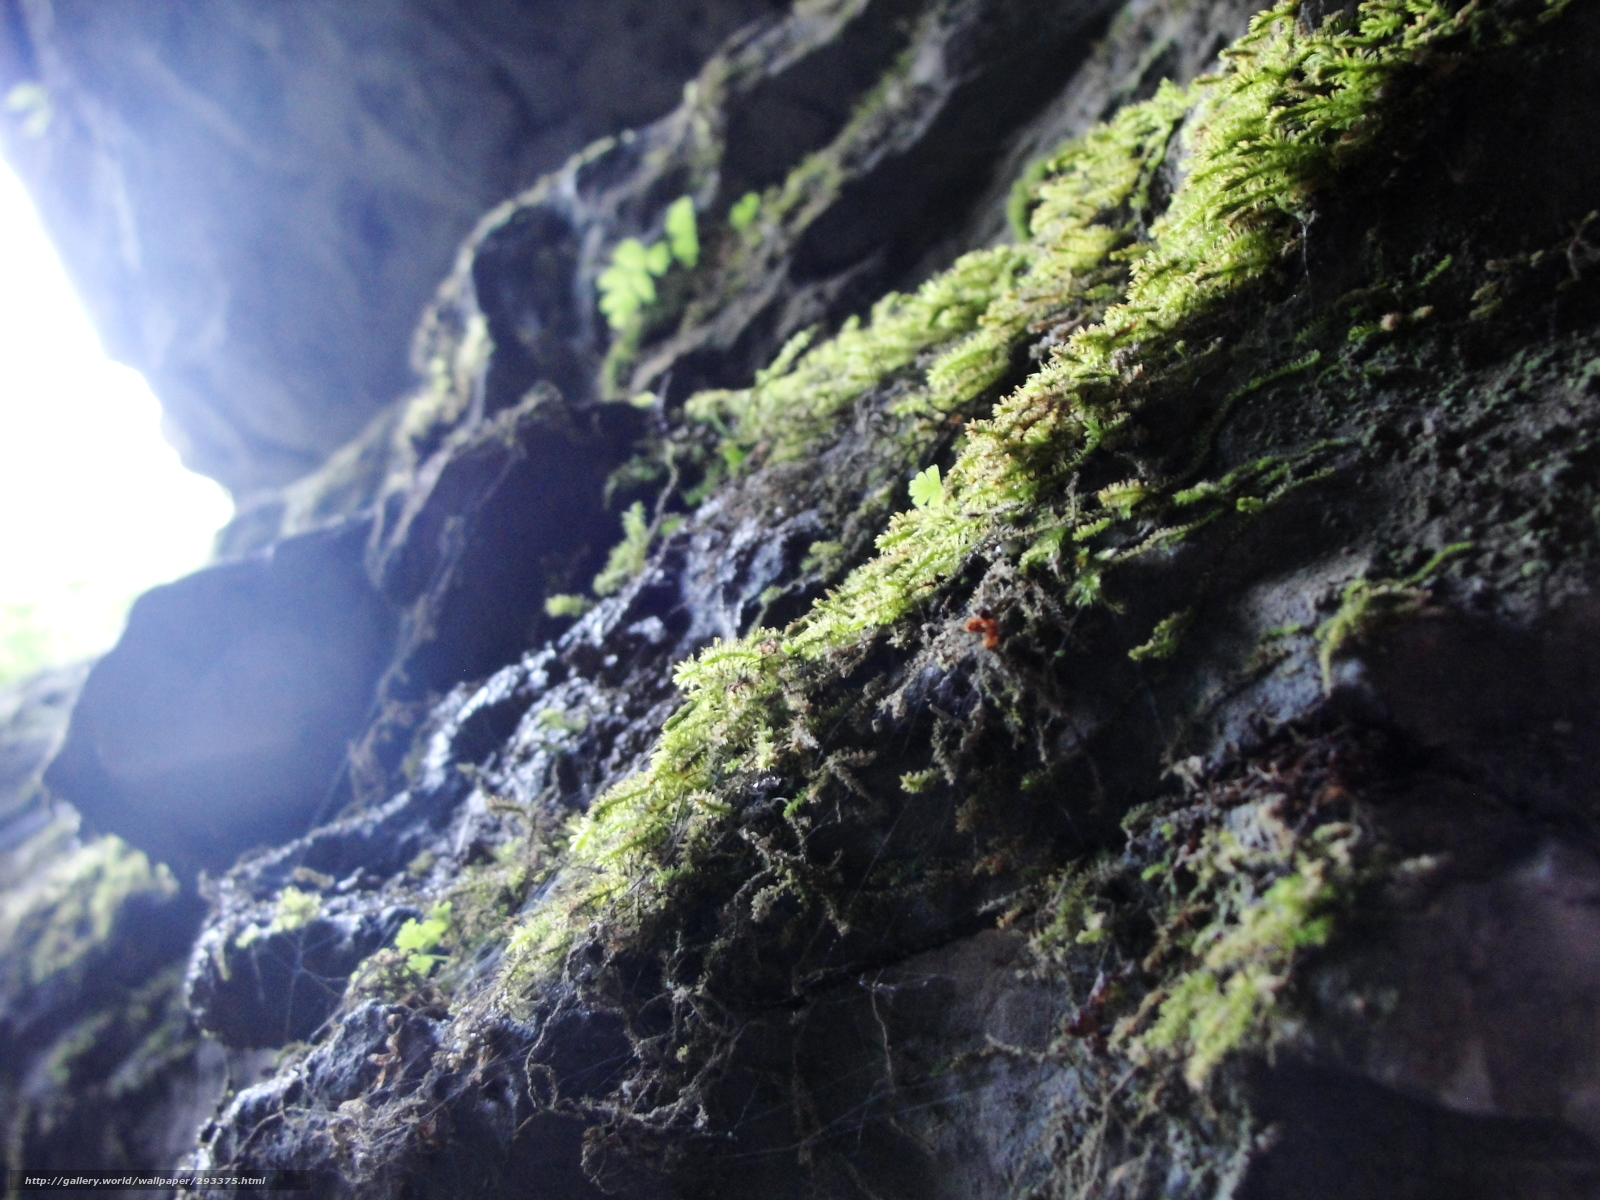
\includegraphics[height=2.2cm,width=1\textwidth,keepaspectratio]{surface_types/moss.jpg}\\
                \caption{Мох}
            \end{subfigure}

            \begin{subfigure}[b]{0.49\textwidth}
                \centering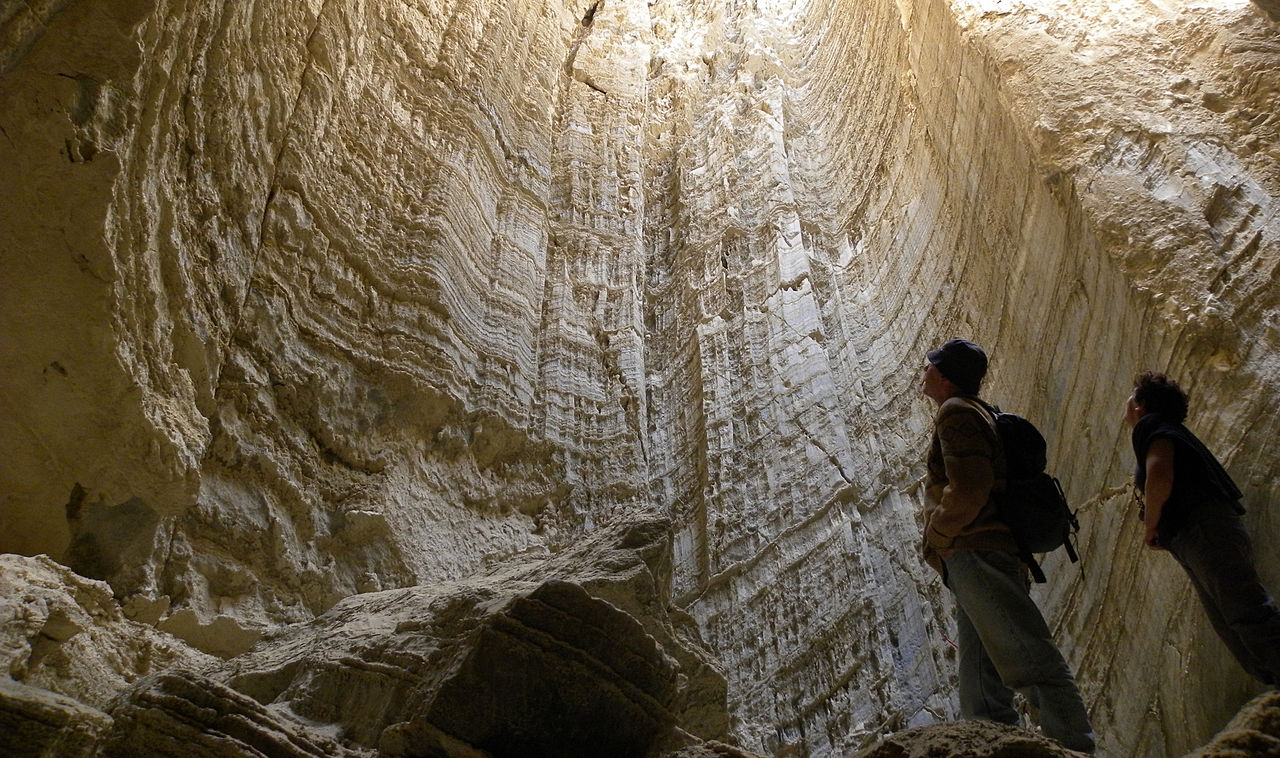
\includegraphics[height=2.0cm,width=1\textwidth,keepaspectratio]{surface_types/salt.jpg}\\
                \caption{Твердые породы}
            \end{subfigure}
            \begin{subfigure}[b]{0.49\textwidth}
                \centering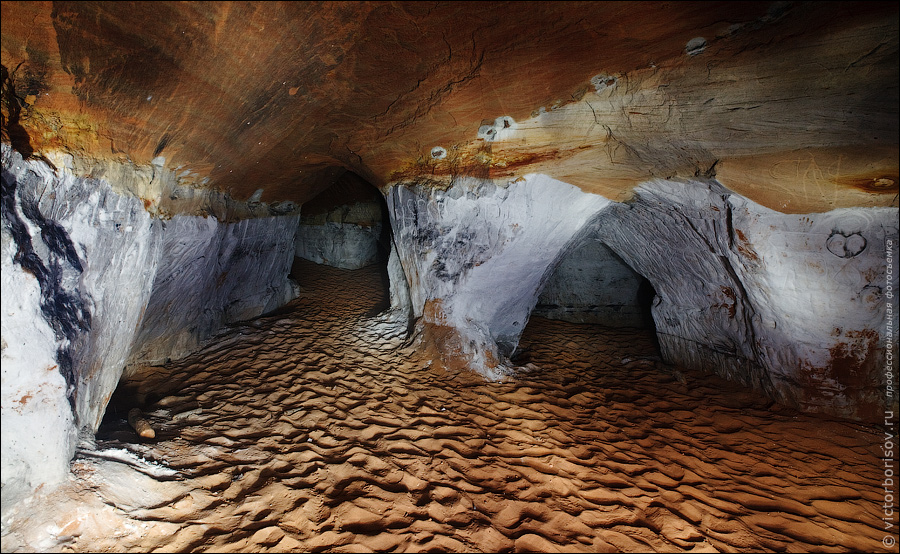
\includegraphics[height=2.0cm,width=1\textwidth,keepaspectratio]{surface_types/sand.jpg}\\
                \caption{Грунт}
            \end{subfigure}
            \caption*{Типы опорных поверхностей}
        \end{subfigure}
        \begin{subfigure}{0.49\textwidth}
            \begin{subfigure}{0.99\textwidth}
                \centering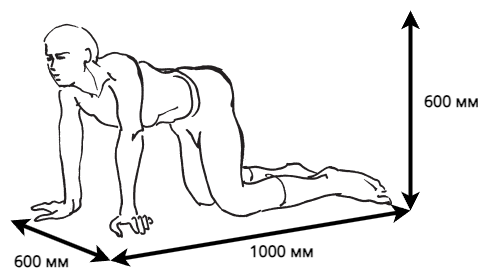
\includegraphics[height=3cm,width=1\textwidth,keepaspectratio]{../images/human_crawling.png}
                \caption*{Габариты пещеры (Свободная узость)}
            \end{subfigure}

            \begin{subfigure}{0.99\textwidth}
                \centering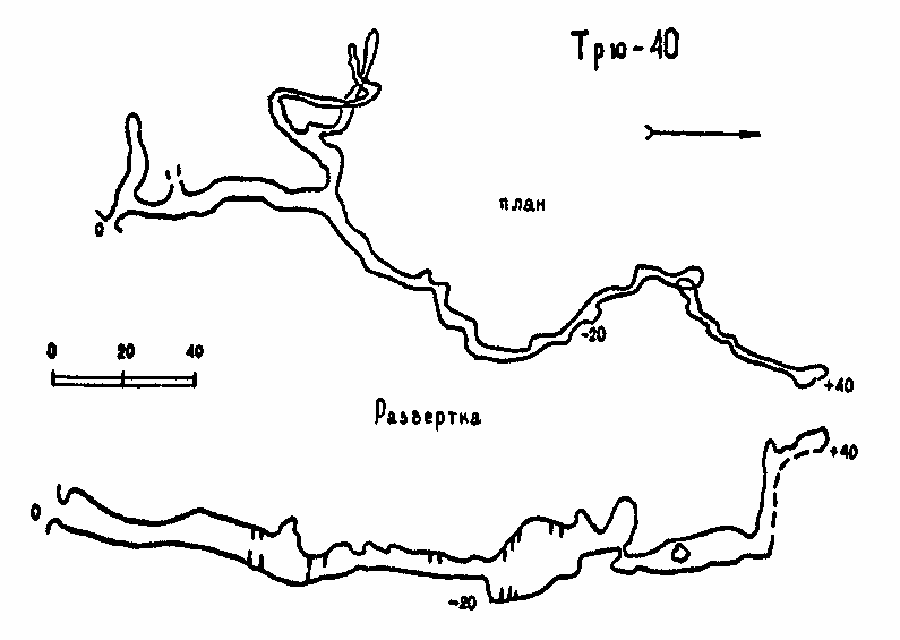
\includegraphics[height=3cm,width=1\textwidth,keepaspectratio]{../images/cave_maps/map3.png}
                \caption*{Протяженность пещер: 1--2 км}
            \end{subfigure}
        \end{subfigure}
    \end{figure}
\end{frame}

\note{\small \setlength{\parindent}{20pt}
\begin{itemize}
    \item Так как пещеры бывают абсолютно разными, я решил ограничить спектр пещер для которых решалась задача. Слева представлены типы опорных поверхностей
    \item Для разработки объекта исследования необходимо понимать также и габариты пещер, а также их протяженность
    \item Глобальная миссия --- разработать робота для исследования пещер.
\end{itemize}
}

% \begin{frame}[t]{Некорректные данные с оптических сенсоров}
%     \framesubtitle{}
%     \begin{figure}[H]
%         \begin{subfigure}[t]{0.49\textwidth}
%             \centering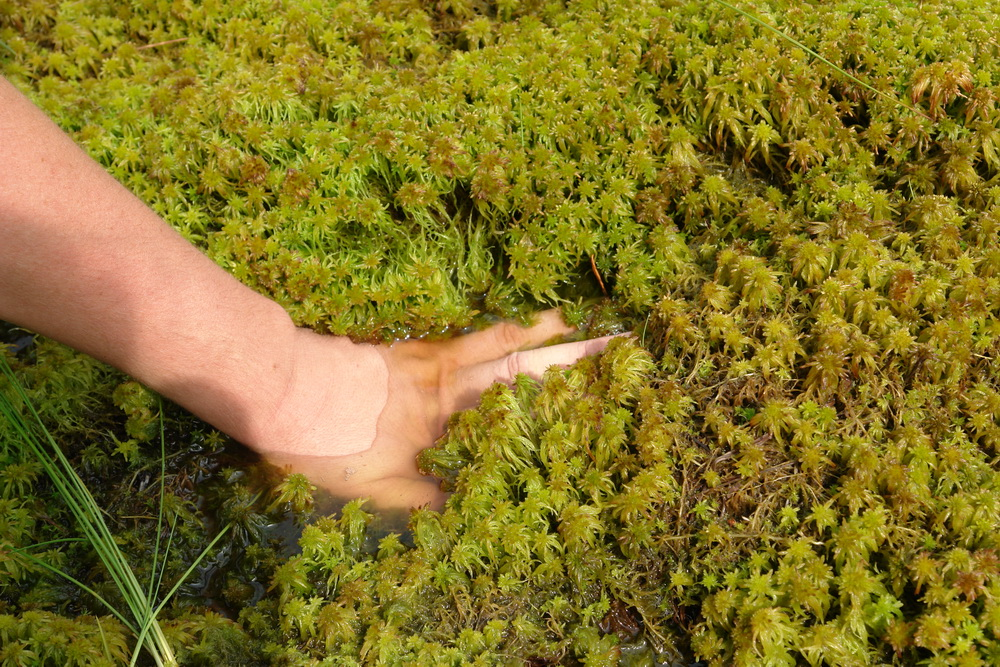
\includegraphics[height=5cm,width=1\textwidth,keepaspectratio]{../images/moh_damping.jpg}
%             \caption*{Мох приминается после ходьбы}
%         \end{subfigure}
%         \begin{subfigure}[t]{0.49\textwidth}
%             \centering\includegraphics[height=5cm,width=1\textwidth,keepaspectratio,page=2]{./tikz_pictures.pdf}
%             \caption*{Лазер отражается от воды, а камера не различает объекты в мутной воде}
%         \end{subfigure}
%     \end{figure}
% \end{frame}

% \note{\small \setlength{\parindent}{20pt}
% Для исследования пещер роботу нужна система навигации. Классические системы навигации основаны на оптических сенсорах.

% К сожалению, в пещерах встречаются случаи, когда оптические сенсоры: лидары, камеры, не смогут достоверно построить карту.

% К примеру, мох *тык*. Он меняет свой объем при наступании на него и это возможно только измерить во время ходьбы. До или после будут уже другой рельеф. 

% Второй пример --- построение опорной поверхности под лужей *тык*. Лидар будет отражаться от поверхности воды и построит гладкую поверхность, а камера не будет работать в мутной воде, как и зеленый лидар.

% С использованием же разработанных методов, данная задача решаема, что и будет показано далее.
% }

\begin{frame}[t]{Цель работы}
    \framesubtitle{}
    Разработать \textbf{метод построения карты местности} с определением \underline{геометрических} и \underline{физико-механических} свойств \textit{опорной поверхности} роботом с шагающими движителями снабженными \underline{тактильными датчиками}, \textit{без использования оптических сенсоров}.
    \begin{figure}[H]
        \begin{subfigure}{0.49\textwidth}
            \centering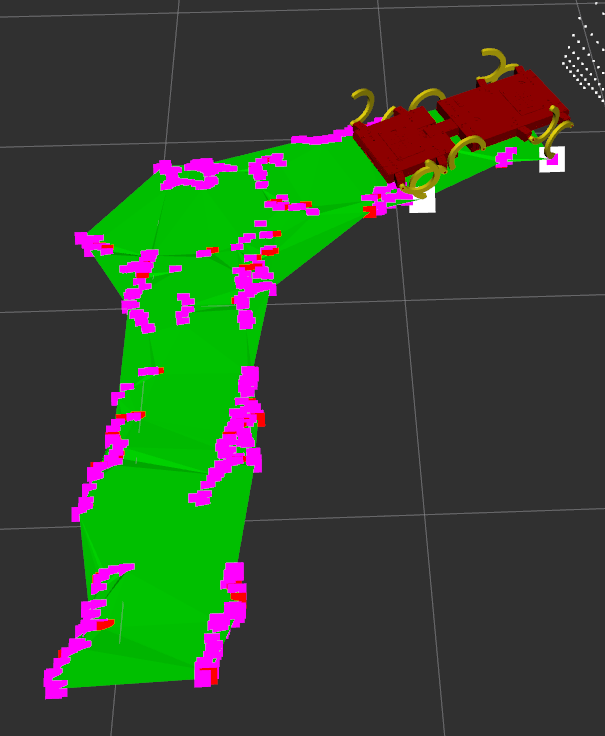
\includegraphics[height=4cm,width=1\textwidth,keepaspectratio]{../images/slides/geom_prop.png}
            \caption*{Определение геометрических свойств}
        \end{subfigure}
        \begin{subfigure}{0.49\textwidth}
            \centering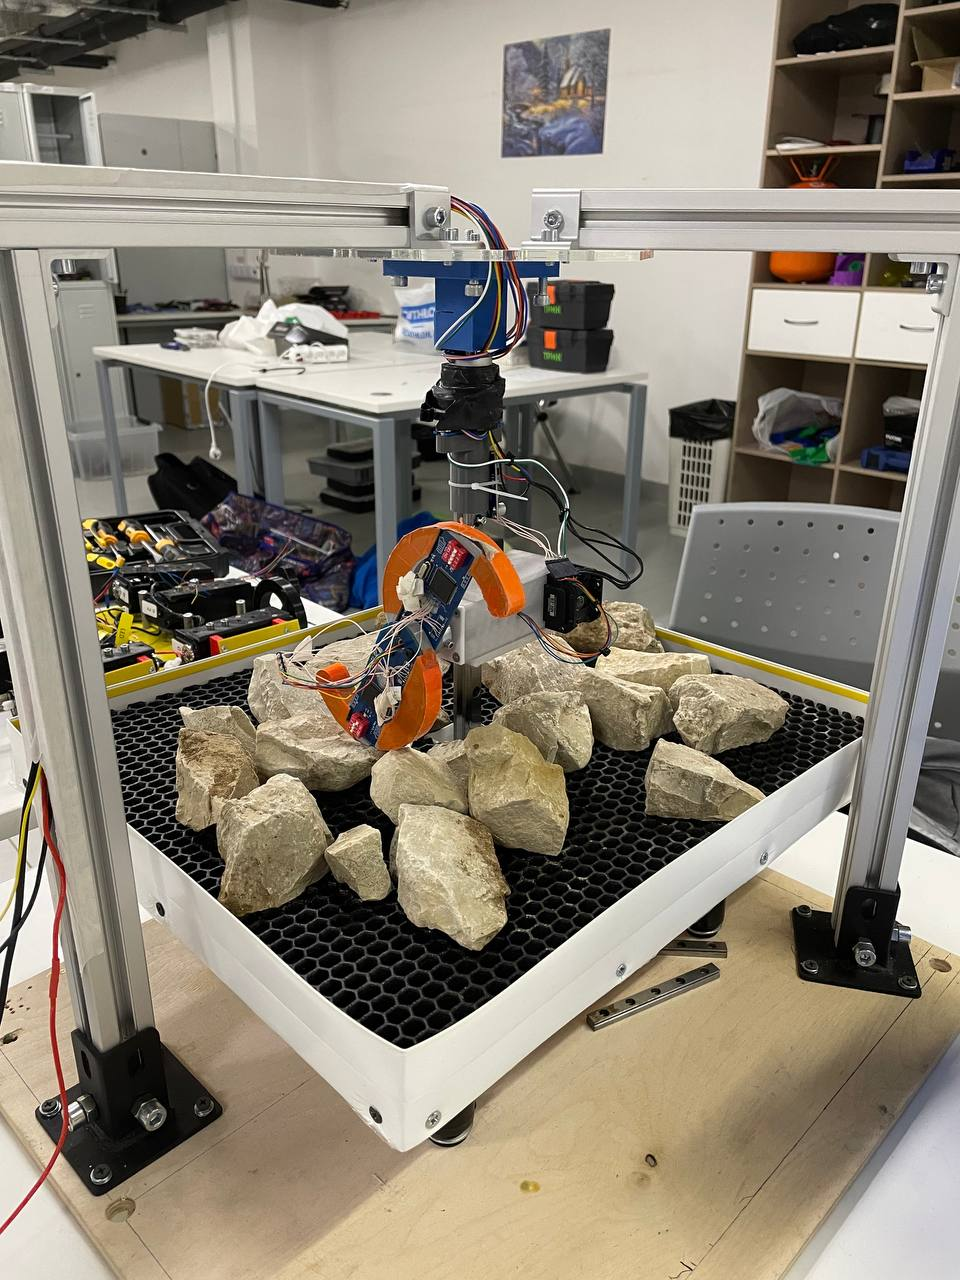
\includegraphics[height=4cm,width=1\textwidth,keepaspectratio]{s_shape_leg/view.jpg}
            \caption*{Определение физических свойств}
        \end{subfigure}
    \end{figure}
\end{frame}

\note{\small \setlength{\parindent}{20pt}
Целью работы являлось разработать метод построения карты местности роботом с шагающими движителями, у которого на стопах установлены датчики силы. Задача должна решаться без использования оптических сенсоров.

Я разбил понятие построения карты на две задачи: определение геометрических свойств *тык* и физико - механических *тык*.

}

\begin{frame}[t]{Построение рельефа местности}
    \framesubtitle{}
    \begin{columns}[T,onlytextwidth]
        \begin{column}{0.49\textwidth}
            \textbf{"4" Геометрические свойства}\\
            \textit{Входные данные}: следовая дорожка, представленная в виде облака точек.

            \textit{Выходные данные}: полигональная сетка и плотное облако точек.
            \vspace{0.35cm}
            \begin{figure}[H]
                \begin{subfigure}[t]{0.49\textwidth}
                    \centering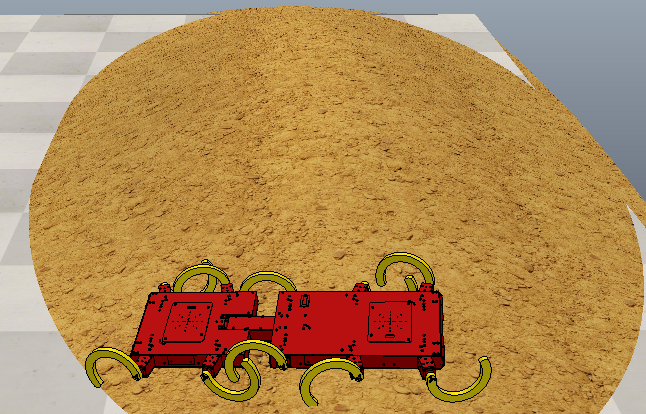
\includegraphics[height=1.9cm,width=1\textwidth,keepaspectratio]{../images/slides/surface_research.png}
                    \caption*{Исследуемая поверхность}
                \end{subfigure}
                \begin{subfigure}[t]{0.49\textwidth}
                    \centering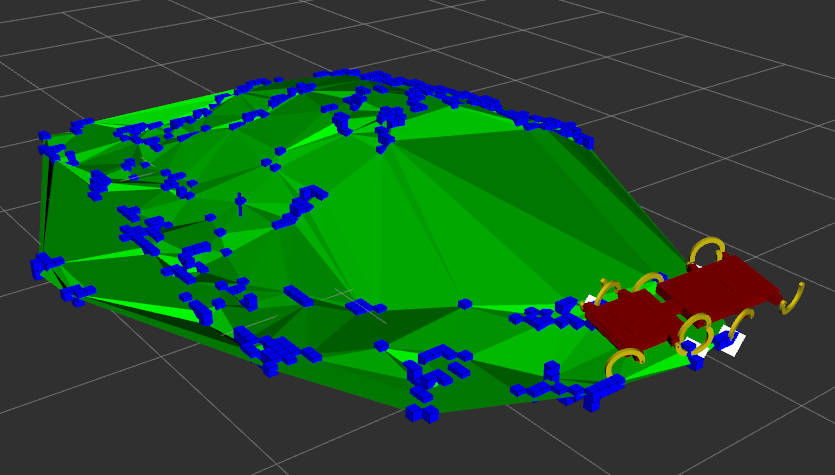
\includegraphics[height=1.9cm,width=1\textwidth,keepaspectratio]{../images/slides/result_research.png}
                    \caption*{Следовая дорожка и полигональная сетка}
                \end{subfigure}
            \end{figure}
        \end{column}
        \begin{column}{0.49\textwidth}
            \textbf{"3" Физико-механические свойства}\\
            \textit{Входные данные}: данные с внутренних датчиков робота.

            \textit{Выходные данные}: процентное соотношение упругих, твердых и пластичных свойств пройденной поверхности.

            \vspace{-0.35cm}
            \begin{figure}[H]
                \begin{subfigure}[t]{0.49\textwidth}
                    \centering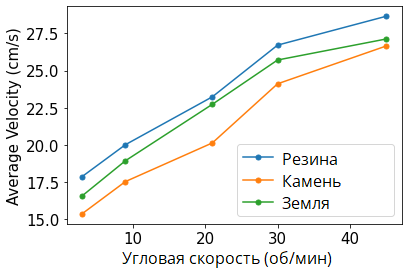
\includegraphics[height=2.5cm,width=1\textwidth,keepaspectratio]{../images/slides/avg_lin_vel_rev_min.png}
                    \caption*{Данные для обучения}
                \end{subfigure}
                \begin{subfigure}[t]{0.49\textwidth}
                    \centering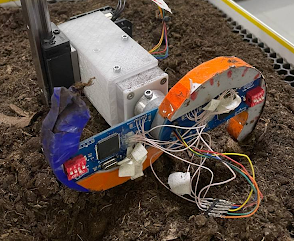
\includegraphics[height=2.5cm,width=1\textwidth,keepaspectratio]{../images/slides/data.png}
                    \caption*{Пример поверхности}
                \end{subfigure}
            \end{figure}
        \end{column}
    \end{columns}
\end{frame}

\note{\small \setlength{\parindent}{20pt}
\begin{itemize}
    \item Задача 4 --- Результатом примененного метода решения должны получиться полигональная сетка пройденной исследуемой поверхности
    \item Задача 3 --- определение какие свойства у пройденной поверхности превалируют: твердые, упругие или пластичные. То есть не всех свойств, а только некоторых
\end{itemize}}

\begin{frame}[t]{Основные научные задачи исследования}
    \framesubtitle{}
    \begin{enumerate}
        \item Разработка метода \textbf{оптимизации конструкции многоногих шагающих роботов} с цикловыми движителями с одной степенью свободы по критериям проходимости, покрытия опорной поверхности и её детализации, длины пройденного пути.
        \item Создание методики \textbf{исследования датчика силы}, когда площадь контакта нажатия на сенсор меньше чувствительной области самого сенсора.
        \item Реализация алгоритма, позволяющего \textbf{определять физические свойства} опорной поверхности.
        \item  Разработка метода \textbf{построения карты местности и определения геометрических свойств поверхности} с помощью тактильного очувствления.
    \end{enumerate}
\end{frame}

\note{\small \setlength{\parindent}{20pt}
\begin{itemize}
    \item Но для решения основных задач, необходимо вначале создать робота и его оптимизировать
    \item Создать датчик и его исследовать
\end{itemize}
}


\begin{frame}{Положения, выносимые на защиту}
    \begin{enumerate}
        \vspace{-0.3cm}
        \small
        \item \textbf{Метод определения физико-механических свойств опорной поверхности} на основе \textbf{тактильного очувствления}, позволяющий различать материалы с \textit{упругими, жёсткими, пластичными свойствами}.
        \item \textbf{Метод построения карты местности}, состоящий в определении геометрической формы поверхности с помощью тактильного очувствления, который позволяет решать задачу определения плана и профиля поверхности в условиях отсутствия видимости и при движении по поверхности, находящейся под водой.
        \item \textbf{Критерий оптимизации} кинематической схемы многоногих шагающих роботов с цикловыми одностепенными движителями, включающий в себя показатели проходимости, покрытия опорной поверхности и её детализации. Определение на его основе габаритов и количества движителей шагающего робота.
        \item \textbf{Зависимость} \textit{погрешности} датчика силы на основе полимерного материала от \textit{площади пятна контакта} относительно размеров датчика, применяемого для тактильного очувствления мобильного робота. \textbf{Методика} роботизированного исследования датчика силы.
    \end{enumerate}
\end{frame}

\note{\small \setlength{\parindent}{20pt}

На защиту выносятся 2 метода, зависимость и критерий оптимизации кинематической схемы}

\begin{frame}[t]{Объект исследования}
    \framesubtitle{}
    \begin{columns}[T,onlytextwidth]
        \begin{column}{0.49\textwidth}
            \textbf{Класс многоногих шагающих роботов} с \\
            а) \underline{Цельным} или \underline{сочленённым} \textit{корпусом}\\
            б) \underline{Цикловыми} \textit{движителями} с \underline{одной степенью свободы}, управляемые зависимо или независимо друг от друга.

            \textit{Требования}:
            \begin{itemize}
                \item Компактные размеры (меньше чем $1000\times600\times600$ мм)
                \item Залезать на препятствия высотой не меньше, чем $\frac{3}{4}$ длины корпуса
                \item Преодолевать представленные
                      опорные поверхности
            \end{itemize}
        \end{column}
        \begin{column}{0.49\textwidth}
            \begin{figure}[H]
                \hfill
                \begin{subfigure}{0.99\textwidth}
                    \centering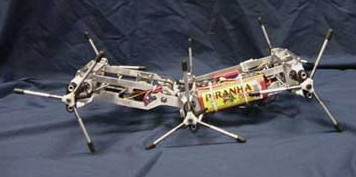
\includegraphics[height=2.5cm,width=1\textwidth,keepaspectratio]{from_master/whegs2.jpg}
                    \caption*{WHegs}
                \end{subfigure}

                \hfill
                \begin{subfigure}[t]{0.49\textwidth}
                    \centering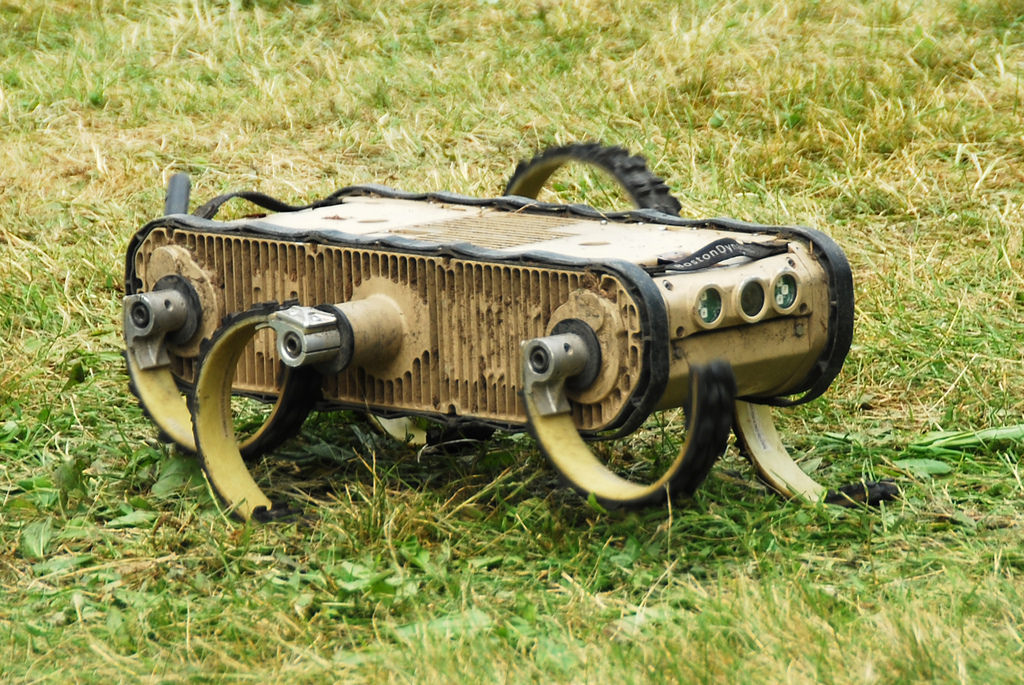
\includegraphics[height=2.5cm,width=1\textwidth,keepaspectratio]{from_master/rhex.jpg}
                    \caption*{Boston Dynamics RHex}
                \end{subfigure}
                \begin{subfigure}[t]{0.49\textwidth}
                    \centering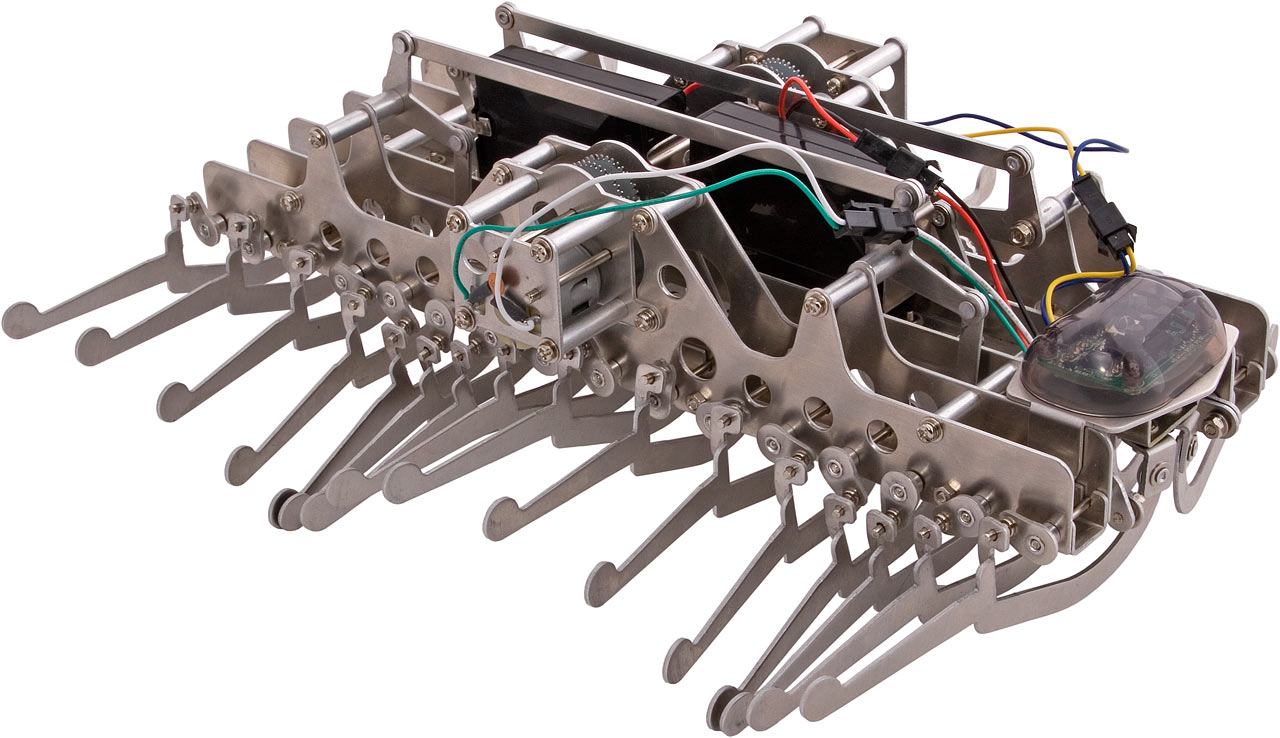
\includegraphics[height=2.5cm,width=1\textwidth,keepaspectratio]{from_master/gakken.jpg}
                    \caption*{Gakken Centipede}
                \end{subfigure}
            \end{figure}
        \end{column}
    \end{columns}
\end{frame}

\note{\small \setlength{\parindent}{20pt}
\begin{itemize}
    \item На основе описания характеристик пещер, мной были выдвинуты требования к объекту исследования
    \item Рассмотрев различные варианты кинематических схем,
    \item В данном видео видно, как подобный класс ...
\end{itemize}
}

\section{Обзор существующих решений}

\begin{frame}[t]{Структура робота}
    \framesubtitle{}
    \begin{figure}[H]
        \centering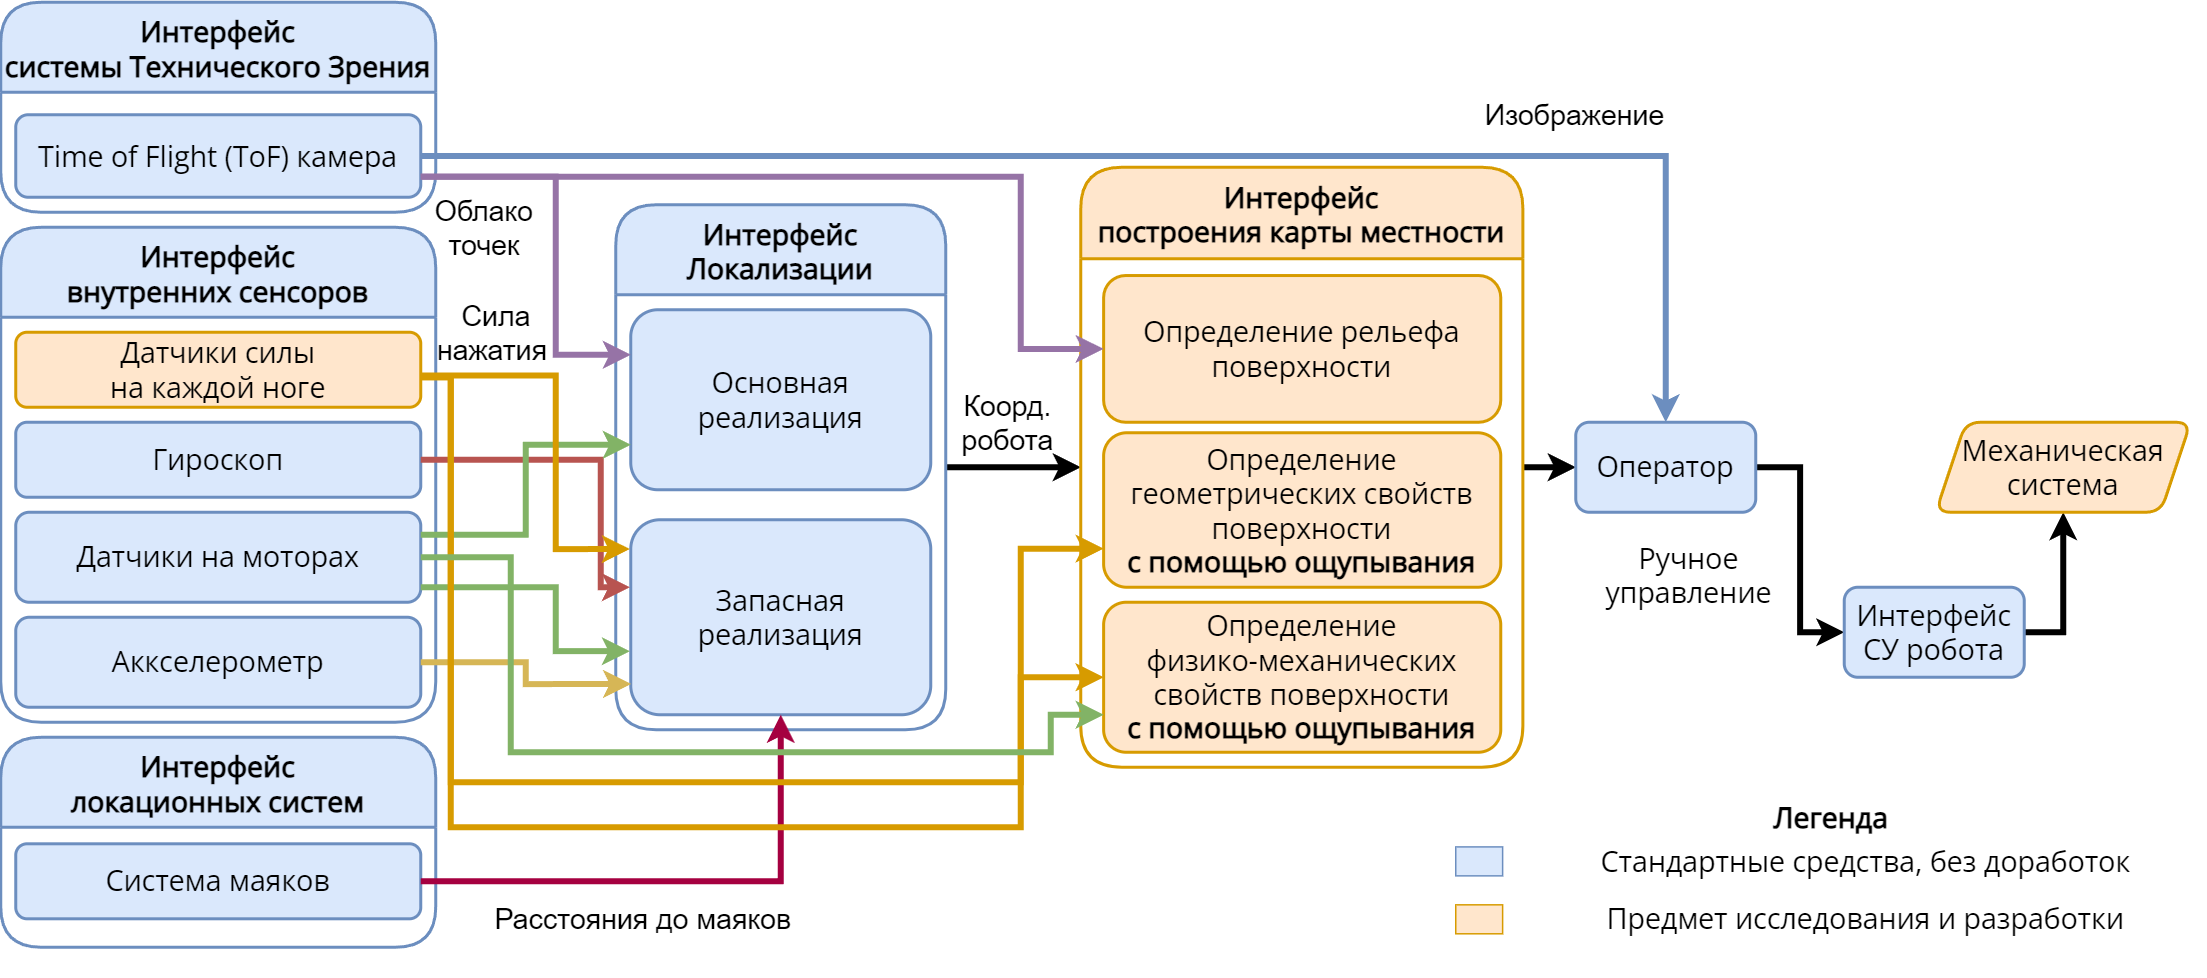
\includegraphics[height=6.5cm,width=1\textwidth,keepaspectratio]{main_diag_hor_new.png}
    \end{figure}
\end{frame}

\note{\small \setlength{\parindent}{20pt}
\begin{itemize}
    \item Робот --- сложная система с множеством подсистем и большую часть подсистем я сам лично не делал.
    \item На слайде *тык* представлена структура проекта
\end{itemize}
}

\begin{frame}[t]{Обзор источников}
    \framesubtitle{}
    \begin{itemize}
        \item \textbf{Задача оптимизации конструкции}: Б. Петриашвили (СССР), Stefano Nolfi (Италия), Dario Sanch-Pradel (Италия), S. Feng (США) и др.
        \item \textbf{Шагающие цикловые роботы}: Е. С. Брискин (Россия), Ю. Д. Андриантов (СССР), Edward Z. Moore (Канада), Wei-Hsi Chen (Китай) и др.
        \item \textbf{Верификация Velostat}:  Igor Vehec (Словакия),  Robert Schroer (США) и др.
        \item \textbf{Определение геометрических свойств поверхности}: Tobias Ebert (Германия), Subodh Kumar (США), И. Рядчиков (Россия), Shan Luo (Британия) и др.
        \item \textbf{Определение физико-механических свойств поверхности}: X. Alice Wu (США), Krzysztof Walas (Польша), Hendrik Kolvenbach (Швейцария) и др.
    \end{itemize}
\end{frame}

\note{\small \setlength{\parindent}{20pt}
\begin{itemize}
    \item При разработке своих подсистем я базировался на работах следующих ученых со всего мира.
    \item Я изучал источники по всем проблемам, которые я озвучил ранее.
    \item Хочу отметить школу шагающих машин Волгограда, на работах и консультациях которых также базируется мое исследование.
\end{itemize}
}